\id{ ҒТАМР \href{https://grnti.ru/?p1=52&p2=47&p3=19}{52.47.19}}{https://doi.org/10.58805/kazutb.v.4.25-637}

\begin{articleheader}

\sectionwithauthors{С.С.Сейтжанов, Н.С.Сүлейменов, П.А.Танжариков, М.Ж.Досжанов, Ғ.Ж.Тасболат}{КЕН ОРНЫНЫҢ САРҚЫЛУЫ ЖАҒДАЙЫНДА МҰНАЙ ҰҢҒЫМАСЫНЫҢ КӨЛДЕНЕҢ
УЧАСКЕСІНІҢ АҒЫМДАҒЫ ҰЗЫНДЫҒЫН АНЫҚТАУ ӘДІСІ}

{\bfseries \textsuperscript{1}С.С.Сейтжанов\textsuperscript{\envelope},
\textsuperscript{1}Н.С.Сүлейменов, \textsuperscript{1}П.А.Танжариков,}

{\bfseries \textsuperscript{2}М.Ж. Досжанов, \textsuperscript{3} Г.Ж.Тасболат}
\end{articleheader}
\begin{affiliation}
\textsuperscript{1}Қорқыт Ата атындағы Қызылорда университеті,
Қызылорда, Қазақстан,

\textsuperscript{2}Қызылорда «Болашақ» университеті, Қызылорда,
Қазақстан,

\textsuperscript{3}Қ.Құлажанов атындағы Қазақ технология және бизнес
университеті, Астана, Қазақстан

\raggedright {\bfseries \textsuperscript{\envelope }}Корреспондент - автор: \href{mailto:seitzhanov_saken@mail.ru}{\nolinkurl{seitzhanov\_saken@mail.ru}}
\end{affiliation}

Ұсақ мұнай кен орындары сарқылуға көлденең ұңғымалармен игерілген кезде,
яғни мұнайды қабаттық қысымды ұстамай-ақ іріктеу жүргізіледі, өйткені
қысымды ұстап тұру үшін қосымша айдау ұңғымаларын бұрғылау қажет.
Қабаттық қысымның қанығу қысымынан төмен түсу диапазонында жоғарыда
аталған коэффициенттердің өзгеруі айтарлықтай болады және бұл ұңғыманың
ағынының төмендеуіне әкеледі. Сондықтан, бастапқы деңгейде жету үшін
қабаттың дебиті мен депрессиясын сақтау үшін көлденең бөліктің ұзындығын
көбейту керек. Көп жағдайда көлденең ұңғымалар көлденең ұңғыманың және
фонтанды құбырларының ұзындығы мен диаметріне, олардың өнімділік
аралығындағы профиліне, ұңғыманың қалыңдығы бойынша орналасуына және
ашылатын қабатшалардың сыйымдылық және сүзу қасиеттерін, кеніш маңындағы
аймақтың ластану дәрежесін, ұңғымаларды суландыру мүмкіндігін және
депрессиялның пайда болуын ескере отырып, дренаж аймағының контурына
қатысты тиісті негіздемесіз бұрғыланады.

Сондықтан көлденең ұңғымалардың таңдағанда, оқпандарды орналастырудан
және ашудың толықтығынан басқа, қабатқа депрессияның мөлшерін,
анизотропия параметрін, өнімді аралықтағы оқпан профилін, сулану
мүмкіндігін және т. б. ескеру қажет.

Көлденең ұңғымалардың конструктивтік ерекшеліктері тік ұңғымалар үшін
әзірленген олардың құрылысын негіздеу әдістері мен технологияларын
тікелей пайдалану, қабаттарды ашу және осындай ұңғымаларды қалыңдығы
бойынша орналастыру мүмкіндігін болдырмайды. Бұл жұмыс осы мәселені
шешуге арналған.

{\bfseries Түйін сөздер:} гидродинамика, қабылдау профилі, кеуекті ортадағы
ағын, қабат, субкапиллярлық канал, мұнай мен газ өндіру, кеуекті орта.

\begin{articleheader}
{\bfseries МЕТОД ОПРЕДЕЛЕНИЯ ТЕКУЩЕЙ ДЛИНЫ ГОРИЗОНТАЛЬНОГО УЧАСТКА НЕФТЯНОЙ
СКВАЖИНЫ В УСЛОВИЯХ ИСТОЩЕНИЯ ЗАЛЕЖИ}

{\bfseries \textsuperscript{1}С.С. Сейтжанов\textsuperscript{\envelope},
\textsuperscript{1}Н.С. Сулейменов, \textsuperscript{1}П.А.Танжариков,}

{\bfseries \textsuperscript{2}М.Ж. Досжанов, \textsuperscript{3}Г.Ж.Тасболат}
\end{articleheader}
\begin{affiliation}

\textsuperscript{1}Кызылординский университет им. Коркыт Ата, Кызылорда,
Казахстан,

\textsuperscript{2}Кызылординский университет «Болашак», Кызылорда,
Казахстан,

\textsuperscript{3}Казахский университет технологии и бизнеса им.
К.Кулажанова, Астана, Казахстан,

е-mail:
\href{mailto:seitzhanov_saken@mail.ru}{\nolinkurl{seitzhanov\_saken@mail.ru}}
\end{affiliation}

При освоении мелких нефтяных месторождений горизонтальными скважинами на
истощение, т. е. без поддержания пластового давления, производится отбор
нефти, так как для поддержания давления необходимо бурение
дополнительных нагнетательных скважин. В диапазоне падения пластового
давления ниже давления насыщения изменение вышеуказанных коэффициентов
будет значительным, и это приведет к снижению расхода скважины. Поэтому
для достижения начального уровня необходимо увеличить длину
горизонтальной части, чтобы сохранить дебит и углубление слоя. В
большинстве случаев горизонтальные скважины бурятся без соответствующего
обоснования длины и диаметра горизонтального ствола и фонтанных труб, их
профиля в пределах продуктивного интервала, расположения ствола по
толщине и относительно контуров зоны дренирования с учетом емкостных и
фильтрационных свойств вскрываемых пропластков, степени загрязнения
призабойной зоны, возможности обводнения скважин и образования глубоких
депрессионных воронок.

Поэтому при выборе конструкции горизонтальных скважин необходимо
учитывать, кроме размещения стволов и полноты вскрытия, величину
депрессии на пласт, параметр анизотропии, профиль ствола в продуктивном
интервале, возможность обводнения и т.д.

Конструктивные особенности горизонтальных скважин исключают возможность
непосредственного использования разработанных для вертикальных скважин
методов и технологий обоснования их конструкции, вскрытия пласта и
размещения таких скважин по толщине. Эта работа предназначена для
решения этой проблемы.

{\bfseries Ключевые слова:} гидродинамика, профиль приемистости, течение в
пористой среде, мощность, субкапиллярный канал, добыча нефти и газа,
пористая среда.
\begin{articleheader}

{\bfseries A METHOD FOR DETERMINING THE CURRENT LENGTH OF A HORIZONTAL
SECTION OF AN OIL WELL UNDER CONDITIONS OF DEPLETION OF A DEPOSIT}

{\bfseries \textsuperscript{1}S.S. Seitzhanov\textsuperscript{\envelope},
\textsuperscript{1}N.S. Suleimenov, \textsuperscript{1}P.A. Tanzharikov,}

{\bfseries \textsuperscript{2}M.Zh. Doszhanov, \textsuperscript{3}G.Zh. Tasbolat}
\end{articleheader}
\begin{affiliation}

\textsuperscript{1}Kyzylorda University named after Korkyt Ata,
Kyzylorda, Kazakhstan,

\textsuperscript{2}Kyzylorda Bolashak University, Kyzylorda, Kazakhstan,

\textsuperscript{3}K. Kulazhanov Kazakh University of Technology and
Business, Astana, Kazakhstan,

е-mail:
\href{mailto:seitzhanov_saken@mail.ru}{\nolinkurl{seitzhanov\_saken@mail.ru}}
\end{affiliation}

When developing small oil fields with horizontal wells for depletion,
i.e. without maintaining reservoir pressure, oil is extracted, since
additional injection wells must be drilled to maintain pressure. In the
range of reservoir pressure drop below the saturation pressure, the
change in the above coefficients will be significant, and this will lead
to a decrease in well flow. Therefore, to reach the initial level, it is
necessary to increase the length of the horizontal part in order to
maintain the flow rate and deepening of the layer. In most cases,
horizontal wells are drilled without an appropriate justification for
the length and diameter of the horizontal trunk and fountain pipes,
their profile within the productive interval, the location of the trunk
in thickness and relative to the contours of the drainage zone, taking
into account the capacitive and filtration properties of the layers
being opened, the degree of contamination of the bottomhole zone, the
possibility of well flooding and the formation of deep depression
funnels.

Therefore, when choosing the design of horizontal wells, it is necessary
to take into account, in addition to the placement of trunks and the
completeness of opening, the amount of depression on the formation, the
anisotropy parameter, the profile of the trunk in the productive
interval, the possibility of watering, etc.

The design features of horizontal wells exclude the possibility of
direct use of methods and technologies developed for vertical wells to
substantiate their design, opening the reservoir and placing such wells
in thickness. This work is designed to solve this problem.

{\bfseries Keywords:} hydrodynamics, pickup profile, flow in a porous
medium, power, subcapillary channel, oil and gas production, porous
medium.
\begin{multicols}{2}

{\bfseries Кіріспе.} Мұнай кен орындарын тік ұңғымалармен игеру кезінде
тордың тығыздығы мен мұндай ұңғымалардың саны газ және газконденсатты
кен орындарын игеру кезінде жасалатындай, мұнайдың тұрақты жылдық
өндірісін сақтауға бағдарланбай белгіленеді. Әдетте, мұнай кен орындарын
игеру процесінде қабаттық қысым іс жүзінде төмендемейтінін атап өткен
жөн, өйткені игеру негізінен қабаттық қысымды ұстап тұру арқылы жүзеге
асырылады, сондықтан мұнай дебитінің төмендеуі негізінен ұңғыманы
айдалатын сумен суландыру нәтижесінде пайда болады. Алайда, Қазақстан
Республикасының аумағында ұңғымалардың саны 3÷5 бірліктен аспайтын
мыңдаған ұсақ мұнай кен орындары бар. Әйтпесе, кен орнын игеру тиімсіз
болып шығады. Мұндай кен орындары әдетте сарқылуға игеріледі, яғни мұнай
алу процесінде айдау ұңғымаларын бұрғылау арқылы қысымды ұстап тұрудың
болмауына байланысты қабат қысымының төмендеуі байқалады. Көбінесе
мұндай кен орындарында олардың мөлшері шектеулі, сондықтан айдау
ұңғымаларын орналастыру оңтайлы болмайды {[}1, 4, 9{]}.

Ұсақ мұнай кен орындары мен көлденең ұңғымалар игерген жағдайда, қабат
қысымының төмендеуі және кеуекті ортаның және оны қанықтыратын мұнайдың
нақты қасиеттерінің өзгеруі жағдайында мұнай мен депрессияның бастапқы
деңгейінде резервуарға шығуын сақтау мүмкіндігі бар.

{\bfseries Материалдар мен әдістер.} Жұмыста {[}1{]} көлденең мұнай
ұңғымаларының өнімділігін анықтау әдістері және осы әдістердің
қолданылуын шектеу шарттары талданады. Бұл әдістердің ішіндегі ең
қолайлысы {[}2{]} және {[}3{]} жұмыстарында ұсынылған әдістер екендігі
көрсетілген.

Жұмысқа {[}1{]} сәйкес тәжірибеге қолайлы дәлдікпен көлденең мұнай
ұңғымасының шығынын келесі формула бойынша анықтауға болады:
\end{multicols}

\begin{equation}
    Q_{\text{көлд.м}} = \frac{kL_{\text{к}} \Delta P}{\mu_{\text{м}} B_{\text{м}} \left[ \frac{1}{h_1} \left( h_1 + R_{\text{с}} \ln \left( \frac{R_{\text{с}}}{R_{\text{с}} + h_1} \right) \right) + \frac{R_{\text{к}} - 2h_1}{4 (R_{\text{с}} + h_1)} \right]}
    \end{equation}
    
 




\begin{figure}[H]
	\centering
	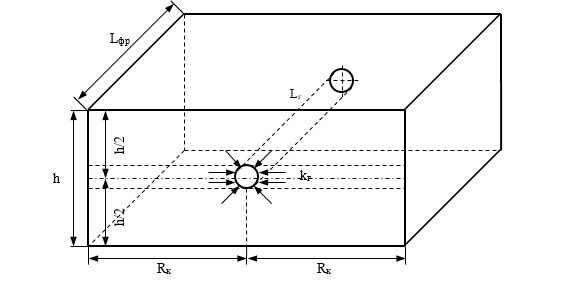
\includegraphics[width=0.6\textwidth]{media/gor/image23.1}
	\caption*{1-сурет. Көлденең оқпанға мұнай ағынының сызбасы}
\end{figure}

\begin{multicols}{2}

мұнда \emph{k} -- қарастырылып отырған жағдайда қабаттың өткізгіштігі
көлденең оқпанға мұнайдың түсуі оқпанға жазық -- радиалды перпендикуляр
және оқпан диаметрінің шегінде ғана көлденең бағытта оған жазық
болатындығына жол беріледі (1-суреті. қара).

Сондықтан, егер қабат анизотропты болса және оның
\emph{k\textsubscript{тік}} тік бағытта өткізгіштігі көлденең бағытта
өткізгіштіктен өзгеше болса, онда (1) формулада
\emph{k\textsubscript{тік}} тік өткізгіштік мәнін қолдану дұрыс болар
еді. Теориялық тұрғыдан алғанда, қабатта айтарлықтай депрессиялар пайда
болған кезде және қабат қысымын төмендету процесінде қабаттың
кеуектілігі мен өткізгіштігі төмендейді. Алайда, бұл өзгерістер көп
жағдайда шамалы, сондықтан пайда болған депрессиядан \emph{k}
өткізгіштігінің өзгеруі және қабат қысымының төмендеуі, яғни
\emph{k=f(∆P,P\textsubscript{қаб.күнд})} өзгеріс аталған жұмыста
ескерілмейді. Анизотропты қабатты ашқан көлденең мұнай ұңғымасының
сенімді өнімділігін формуланы (1) келесі тәуелділікпен ауыстыру арқылы
анықтауға болады:


\end{multicols}
\begin{equation}
    Q_{\text{көлд.м}} = \frac{kL_{\text{к}} \Delta P}{\mu_{\text{м}} B_{\text{м}} \left[ \frac{1}{v h_1} \left( \nu h_1 + R_{\text{с}} \ln \frac{R_{\text{с}}}{R_{\text{с}} + v h_1} \right) + \frac{R_{\text{к}} - 2v h_1}{4 (R_{\text{с}} + v h_1)} \right]}
    \end{equation}
    
    \begin{multicols}{2}

мұнда \emph{v --} мына теңдіктен анықталған анизотропия параметрі:
\emph{v=}{[}\emph{k\textsubscript{т}/k}\textsubscript{к}{]}\emph{\textsuperscript{0,5}},
\emph{k\textsubscript{т}, k}\textsubscript{к} - тік және көлденең
бағыттардағы өткізгіштік коэффициенттері; \emph{L}\textsubscript{к} -
\emph{R\textsubscript{с}} радиусымен оқпанның көлденең бөлігінің
ұзындығы; \emph{∆P} --
\emph{∆P=Р\textsubscript{қаб}-Р\textsubscript{түп}},
\emph{Р\textsubscript{қаб}}, \emph{Р\textsubscript{түп}} тең қабатқа
депрессия -- тиісінше, дренаж аймағының контурындағы және ұңғыманың түп
аймағындағы қысым. Айта кету керек, жұмыста талданған көлденең мұнай
ұңғымаларының өнімділігін анықтаудың барлық әдістері {[}1{]} көлденең
бағананың ұзындығы бойынша тұрақты түп қысыммен ғана жарамды, яғни
\emph{Р\textsubscript{түп}}=const болғанда, \emph{µ\textsubscript{м}} --
қабат жағдайындағы мұнайдың тұтқырлық коэффициенті;
\emph{В\textsubscript{м}} -- мұнайдың көлемдік коэффициенті яғни қабат
жағдайындағы мұнай көлемінің стандартты жағдайдағы көлемге қатынасы;
\emph{h\textsubscript{1}} - келесі теңдіктен қабылданған есептеу схемасы
үшін анықталған қабаттың қалыңдығы:
\emph{h\textsubscript{1}=h/h\textsubscript{2}-R\textsubscript{c}}, егер
ұңғыма оқпаны қабаттың қалыңдығына симметриялы орналасса;
\emph{R\textsubscript{к}} -- дренажды ұңғымамен аймақтың шекарасына
дейінгі қашықтық.

Көлденең оқпанмен полосообразды қабаттың толық ашылуымен мұнайдың
шығынын салыстырмалы түрде сенімді анықтауға мүмкіндік беретін {[}1{]}
және {[}2{]} жұмыстарында ұсынылған әдістер (1-сур. қар.).

{\bfseries Нәтижелер және талқылау.} З.С. Алиев пен В.В. Шеремет ұсынған
(1), (2) формулалардан және {[}1{]} көлденең мұнай ұңғымасының дебитін
анықтау үшін келтірілгеннен, қабаттағы белгілі депрессияда, мұнай
\emph{µ\textsubscript{м}} және \emph{В\textsubscript{м}} қасиеттерін,
сонымен қатар дренаж аймағының геометриясын ені бойынша
\emph{L\textsubscript{к}} көлденең учаскенің ұзындығының әртүрлі
мәндерімен беру керек. Осы формуланы қолдана отырып, көлденең бөліктің
ұзындығын анықтауға болады. Анизотропты қабат үшін көлденең учаскенің
ұзындығы келесідей болады:

\end{multicols}
\begin{equation}
    L_{\text{к}} = \frac{Q_{\text{көлд.м}} \mu_{\text{м}} B_{\text{м}} \left[ \frac{1}{v h_1} \left( \nu h_1 + R_{\text{с}} \ln \frac{R_{\text{с}}}{R_{\text{с}} + v h_1} \right) + \frac{R_{\text{к}} - 2v h_1}{4 (R_{\text{с}} + v h_1)} \right]}{k \Delta P}
    \end{equation}
    
    \begin{multicols}{2}

Егер мұнай кен орындары массивті болса және бұрын айтылғандай сарқылу
үшін жасалса, олар тіпті бір артық пайдалану ұңғымасын бұрғылау кезінде
табан суының көтерілуіне байланысты олардың игеру рентабельділігін күрт
нашарлатады, содан кейін мұнай өндіру процесінде мұнаймен қаныққан h(t)
қалыңдығы, сәйкесінше, \emph{h\textsubscript{1}}(t) қалыңдығы
төмендейді. Сонымен қатар, қабат қысымының төмендеуіне байланысты
\emph{µ\textsubscript{м}}(\emph{Р}) және
\emph{В\textsubscript{м}}(\emph{Р}) мұнай қасиеттерінің өзгеруі
байқалады. \emph{h\textsubscript{1}}(t) және
\emph{µ\textsubscript{м}}(\emph{Р}), \emph{В\textsubscript{м}}(\emph{Р})
мүмкін болатын өзгерістерін ескере отырып, бастапқы қысым кезінде
анықталған мұнай қасиеттерімен қабаттағы депрессияның бастапқы
мәндерінде және бастапқы қабат қысымында алынған мұнайдың бастапқы
дебитін қамтамасыз ету үшін көлденең учаскенің ұзындығын келесі формула
бойынша анықтау қажет {[}4{]}:
\end{multicols}


\begin{equation}
    L_{\text{к}}(t) = \frac{Q_{\text{көлд.м.бас}} \mu_{\text{м}}(P) B_{\text{м}}(P) \left[ \frac{1}{v h_1(t)} \left( \nu h_1(t) + R_{\text{с}} \ln \frac{R_{\text{с}}}{R_{\text{с}} + v h_1(t)} \right) + \frac{R_{\text{к}} - 2v h_1(t)}{4 (R_{\text{с}} + v h_1(t))} \right]}{k \Delta P}
    \end{equation}
    \begin{multicols}{2}
    
Бұл параметрлердің өзгеру сипаты қысымнан және уақыт бойынша, атап
айтқанда, мұнайдың қасиеттері мұнайдың газбен қанығу қысымының мөлшеріне
байланысты. Салыстырмалы түрде төмен қанықтыру қысымында
\emph{µ\textsubscript{м}}(\emph{Р}) мен
\emph{В\textsubscript{м}}(\emph{Р}) коэффициенттері дамудың бірінші
кезеңінде, яғни
\emph{Р\textsubscript{қабат}}\textgreater{}\emph{Р\textsubscript{қанық}}
қабат қысымы қанығу қысымына дейін төмендегенге дейін тұрақты болып
қалады. Мұнайдың газбен қанығуының төмен қысымы мұнай кен орындарында
бос газ болмаған кезде және газ қақпағы бар кен орындарында бұл газ жоқ
аймақтарда орын алатынын атап өтеміз.

Қысымнан мұнайдың тұтқырлығының өзгеруін
\emph{µ\textsubscript{м}}(\emph{Р}) шамамен формула бойынша анықтауға
болады:

\begin{equation}
    \mu_{\text{м}}(P) = \mu_{\text{м.қаб}} + \frac{\delta(P_{\text{қабат}} - P_{\text{қанық}})}{P_{\text{аm}}}
    \end{equation}
  

мұнда \emph{µ\textsubscript{м}}(\emph{Р}) --
\emph{Р\textsubscript{қабат}}\textgreater{}\emph{Р\textsubscript{қанық}}
аясындағы \emph{Р\textsubscript{қабат}}(t) мен
\emph{Т\textsubscript{қабат}} кезіндегі мұнайдың тұтқырлығы;
\emph{µ\textsubscript{м.қабат.бас }}-- \emph{Р\textsubscript{қанық}}
қанықтыру қысымындағы қабаттағы мұнайдың тұтқырлығы; \emph{δ} -- мұнай
тұтқырлығы мен қабат қысымы арасындағы пропорционалдылық коэффициенті
1-кестеде келтірілген қысымның өзгеру диапазонының келесі мәндерінің
қысымына байланысты анықталады {[}5, 6{]}.

\end{multicols} 


\begin{longtable}[]{|@{}
    >{\raggedright\arraybackslash}p{(\columnwidth - 4\tabcolsep) * \real{0.0554}}|
    >{\raggedright\arraybackslash}p{(\columnwidth - 4\tabcolsep) * \real{0.3599}}|
    >{\raggedright\arraybackslash}p{(\columnwidth - 4\tabcolsep) * \real{0.5848}}|@{}}
    \caption*{1-кесте. Мұнайдың тұтқырлығы мен қабат қысымы арасындағы
пропорционалдылық коэффициентінің тәуелділігі} \\
  \hline
  \begin{minipage}[b]{\linewidth}\raggedright
  р/с
  \end{minipage} & \begin{minipage}[b]{\linewidth}\raggedright
  Мұнай тұтқырлығының өзгеру диапазоны \emph{µ\textsubscript{м}}(\emph{Р})
  мПа
  \end{minipage} & \begin{minipage}[b]{\linewidth}\raggedright
  \emph{Т\textsubscript{қабат}} және \emph{Р\textsubscript{қанық}} кезінде
  \emph{δ} пропорционалдылық коэффициентін анықтау формуласы
  \end{minipage} \\ \hline
  \endfirsthead
  \hline
  \begin{minipage}[b]{\linewidth}\raggedright
  р/с
  \end{minipage} & \begin{minipage}[b]{\linewidth}\raggedright
  Мұнай тұтқырлығының өзгеру диапазоны \emph{µ\textsubscript{м}}(\emph{Р})
  мПа
  \end{minipage} & \begin{minipage}[b]{\linewidth}\raggedright
  \emph{Т\textsubscript{қабат}} және \emph{Р\textsubscript{қанық}} кезінде
  \emph{δ} пропорционалдылық коэффициентін анықтау формуласы
  \end{minipage} \\ \hline
  \endhead
  \hline
  \endfoot
  \endlastfoot
  1 & 0 ≤ \emph{µ\textsubscript{м}}(\emph{Р}) ≤ 5 & \emph{δ =} 0,00114
  {[}\emph{µ\textsubscript{қабат}}(\emph{Р\textsubscript{қанық}}){]} \\ \hline
  2 & 5 ≤ \emph{µ\textsubscript{м}}(\emph{Р}) ≤ 10 & \emph{δ =}
  0,057+0,023
  {[}\emph{µ\textsubscript{қабат}}(\emph{Р\textsubscript{қанық}}) - 5{]} \\ \hline
  3 & 10 ≤ \emph{µ\textsubscript{м}}(\emph{Р}) ≤ 25 & \emph{δ =}
  0,171+0,031
  {[}\emph{µ\textsubscript{қабат}}(\emph{Р\textsubscript{қанық}}) - 10{]} \\ \hline
  4 & 25 ≤ \emph{µ\textsubscript{м}}(\emph{Р}) ≤ 45 & \emph{δ =}
  0,643+0,045
  {[}\emph{µ\textsubscript{қабат}}(\emph{Р\textsubscript{қанық}}) - 25{]} \\ \hline
  5 & 45 ≤ \emph{µ\textsubscript{м}}(\emph{Р}) ≤ 75 & \emph{δ =}
  1,539+0,058
  {[}\emph{µ\textsubscript{қабат}}(\emph{Р\textsubscript{қанық}}) - 45{]} \\ \hline
  6 & 75 ≤ \emph{µ\textsubscript{м}}(\emph{Р}) ≤ 85 & \emph{δ =}
  3,286+0,100
  {[}\emph{µ\textsubscript{қабат}}(\emph{Р\textsubscript{қанық}}) - 75{]} \\ \hline
  \end{longtable}
  



\begin{figure}[H]
	\centering
	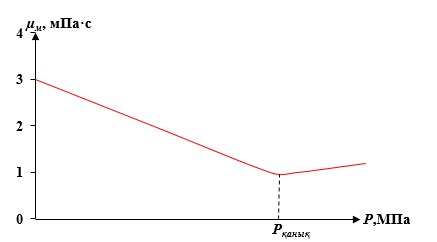
\includegraphics[width=0.6\textwidth]{media/gor/image23.2}
	\caption*{ 2-сурет. Мұнайдың тұтқырлығының \emph{µ\textsubscript{м}}
    қысымға тәуелділігі}
\end{figure}

\begin{multicols}{2}

Мұнайдың тұтқырлығының \emph{µ\textsubscript{н}} қысымға тәуелділігінің
классикалық түрі 2-суретте көрсетілген.

Суреттен көріп тұрғанымыздай, \emph{Р\textsubscript{қабат}} қабат қысымы
\emph{Р\textsubscript{қанық}} қанығу қысымынан жоғары болғанда, мұнайдың
тұтқырлығының өзгеруі мұнай газсыздандырылатын
\emph{Р\textsubscript{қабат}\textless Р\textsubscript{қанық}} аймағына
қарағанда аз қарқынды. Мұнайда еріген газдың мөлшері азайған сайын
мұнайдың тұтқырлығы қарқынды өседі. 3-суретте мұнайдың тұтқырлығының әр
түрлі температурада еріген газ мөлшерінен эмпирикалық тәуелділігі
көрсетілген.
\end{multicols}


\begin{figure}[H]
	\centering
	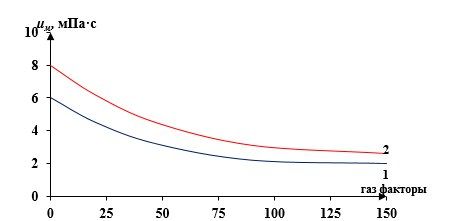
\includegraphics[width=0.6\textwidth]{media/gor/image23.3}
	\caption*{  3-сурет. 1- Т=60\textsuperscript{0}С; 2-
    Т=40\textsuperscript{0}С темратурасында еріген газ мөлшерінен
    \emph{µ\textsubscript{м}} мұнай тұтқырлығының тәуелділігі}

\end{figure}

\begin{multicols}{2}

(1) және (2) формулаларында \emph{В\textsubscript{м}} арқылы белгіленген
көлемді мұнай коэффициенті қабат жағдайындағы мұнай көлемінің стандартты
жағдайдағы көлемге қатынасын білдіреді. Себебі қалыпты жағдайларда
мұнайда еріген газ жоқ, сондықтан мұнай көлемі еріген газдың бірдей
мөлшерінен аз болады. Сәйкесінше мұнайдың \emph{В\textsubscript{м}}
көлемді коэффициенті қашан да бірліктен үлкен болады.
\emph{В\textsubscript{м}} мұнайдың көлемді коэффициенті келесі теңдікпен
анықталады {[}7 - 10{]}:

\begin{equation}
    V_{\text{м}} = \frac{V_{\text{м.қабат}}}{V_{\text{м.жағд}}}
    \end{equation}
    

мұнда \emph{V\textsubscript{м.қабат}} және
\emph{V\textsubscript{м.жағд}} -- тиісінше, қабаттағы және қалыпты
жағдайдағы мұнай көлемі. Қазақстан Республикасында есептеу
формулаларында көлемдік коэффициент жоқ екенін атап өткен жөн, өйткені
бұл формулаларда қалыпты жағдайлардағы мұнай көлемі қарастырылған.

Жоғарыда айтылғандардан, егер даму процесінде қабат қысымының төмендеуі
байқалса және осы орайда қысым аймағында қысымнан төмен болса, көлемдік
коэффициент азаяды және мұнайдың тұтқырлығы артады, сонымен қатар
мұнаймен қаныққан қабат қалыңдығы азаяды. (1) және (2) формулалардағы
көлденең мұнай ұңғымасының дебиті мен мұнайдың тұтқырлығы, көлемдік
коэффициенті мен мұнайға қаныққан аралықтың қалыңдығы арасындағы
тәуелділіктерден бұл параметрлердің өзгеруі мұнай дебитінің төмендеуіне
әкелетінін көреміз. Осы өзгерістер кезінде мұнай шығынын сақтау үшін
оқпанның көлденең бөлігінің ұзындығын арттыру қажет. Мұндай ұзындықты
осы жұмыста ұсынылған (4) формуламен анықтауға болады.

{\bfseries Қорытынды.} Қорытындылай келе, авторлар қабаттық қысымның газбен
қанығу қысымының шамасына дейін төмендеуімен тұтқырлық пен көлемдік
коэффициенттің өзгеруі өте аз екенін және көлденең учаскенің ағымдағы
ұзындығы \emph{L}\textsubscript{к}(t) негізінен мұнаймен қаныққан
интервалдың қалыңдығының өзгеруімен алдын-ала анықталатынын және егер
қабаттың мұнаймен қаныққан қалыңдығының өзгеруі шамалы болса, онда
көлденең оқпанның ағымдағы ұзындығы бастапқы ұзындығынан сәл өзгеше
болатындығын тағы бір мәрте атап өтеді.

Оқпанның көлденең бөлігінің ұзындығының едәуір өсуі қабаттың қысымы
қанығу қысымынан төмен аймақта орын алады. Сондықтан көлденең
ұңғымаларды қолдана отырып, шағын қорлары бар мұнай кен орындарын
игеруді жобалау барысында, қабаттық қысымды ұстап тұру үшін айдау
ұңғымаларын бұрғылау мұндай кен орындарын игерудің рентабельділігін күрт
төмендеткен кезде, \emph{L}\textsubscript{к}(t) оқпанның көлденең
бөлігінің ағымдағы ұзындығын анықтау кезінде кеуекті орта мен мұнай
қасиеттерінің өзгеруін ескеру қажет.

Кен орнының сарқылуы жағдайында мұнай ұңғымасының көлденең учаскесінің
ағымдағы ұзындығын салыстыру үшін аталған жұмыста жоғарыда аталған
әдістерге келесі бастапқы мәндер қолданылды:
\emph{R\textsubscript{к}}=400 м; \emph{R\textsubscript{с}}=0,1м;
\emph{k}=0,15 Дарси; \emph{В\textsubscript{м}}=1,25 және 1,1;
\emph{μ\textsubscript{м}}=0,5 и 1 мПа·с;
\emph{Q\textsubscript{көлд.м}}=300 м\textsuperscript{3}/тәул;
\emph{h\textsubscript{2}}=25 және 30 м \emph{L\textsubscript{көлд}.}

(1) және (2) формулалардағы көлденең мұнай ұңғымасының дебиті мен
мұнайдың тұтқырлығы, көлемдік коэффициенті мен мұнайға қаныққан
аралықтың қалыңдығы арасындағы тәуелділіктерден бұл параметрлердің
өзгеруі оқпанның көлденең бөлігінің ұзындығының ұлғаюына әкелетінін
көрсетеді. Мысалы, (4) формула бойынша \emph{Q\textsubscript{м}}=300
м\textsuperscript{3}/тәул кезінде мұнай тұтқырлығының
\emph{μ\textsubscript{м}} =0,5-тен 1 мПа·с дейін артуында,
\emph{L\textsubscript{көлд }}көлденең оқпанның ұзындығы 553,2 м-ден
608,5 м-ге дейін артады. Қабат қалыңдығының \emph{h}=25 м-ден
\emph{h}=30 м-ге, яғни в 1,2 есе артуы, \emph{L\textsubscript{көлд}}
көлденең оқпанның ұзындығын \emph{L\textsubscript{көлд}=}713,9 м-ден
\emph{L\textsubscript{көлд}=}608,5 м-ге әкеледі.

Түп қысымы мұнайдың газбен қанығу қысымының шамасына дейін төмендеген
кезде тұтқырлық пен көлемдік коэффициенттің өзгеруі өте аз болатындығы
және көлденең учаскенің ағымдағы ұзындығы негізінен мұнаймен қаныққан
интервалдың қалыңдығының өзгеруімен алдын-ала белгіленетіні анықталды.
Сондықтан бастапқы деңгейде қабаттың дебиті мен депрессиясын сақтау үшін
көлденең учаскенің ұзындығын көбейтіп отыру қажет.
\end{multicols}

\begin{center}
	{\bfseries Әдебиеттер}
	\end{center}
	
	\begin{references}

1. Алиев З.С., Бондаренко В.В., Сомов Б.Е. Методы определения
производительности горизонтальных нефтяных скважин и параметров вскрытых
ими пластов. - М.: Изд. Нефть и газ, 2001. - С.15-18. ISBN:
5-7246-0162-1

2. Алиев З.С., Шеремет В.В. Определение производительности
горизонтальных скважин, вскрывших газовые и газонефтяные пласты. - М.:
Изд. Нефть и газ, 1995, С.64-68. ISBN 5-247-03534-8.

3. Алиев З.С., Сомов Б.Е., Чекушин В.Ф. Обоснование конструкции
горизонтальных и многоствольно-горизонтальных скважин для освоения
нефтяных месторождений. -М.: Издательство «Техника». ООО «ТУМА ГРУПП»,
2001.-192 с. ISBN 5-93969-011-4

4. Сейтжанов С.С. Диссертация «Разработка методов обоснования
производительности горизонтальных нефтяных скважин при различных формах
зоны дренирования». -- РГУ нефти и газа (НИУ) им. И. М. Губкина, 2011. -
144 c. URL: \url{https://www.dissercat.com}

5. Сейтжанов С.С., Сүлейменов Н.С., Ахметов Н.Х. Табаны сулы кенішті
ашқан горизонталь оқпанды мұнай ұңғымасының шектік сусыз өнімін анықтау
әдістемесі //НЕФТЬ И ГАЗ . --2023. --№ 5 (137). - С.107-114. DOI:
10.37878/2708-0080/2023-5.06

6. Сейтжанов С.С., Сүлейменов Н.С., Танжариков П.А. Қарашығанақ мұнай
кен орнындағы горизонтальды ұңғымалардың өнімділігіне әсер ететін
факторлар //НЕФТЬ И ГАЗ. -2023. -№. 6 (138). -С.151-159. DOI:
10.37878/2708-0080/2023-6.14

7. Серикбаев Е.А., Сейтжанов С.С., Сулейменов Н.С., Танжариков П.А.,
Абильдаев Н.A. Көлденең оқпанның арасындағы арақашықтықтың мұнай
ұңғымаларының өнімділігіне әсері // НЕФТЬ И ГАЗ. -2024. --№2 (140).
-С.81-92 \href{https://doi.org/10.37878/2708-0080/2024-2.08}{DOI:
10.37878/2708-0080/2024-2.08}

8. Сейтжанов С.С., Сулейменов Н.С., Танжариков П.А., Құрбанов Н.A. Қабат
анизотропиясының әр түрлі параметрлері кезіндегі горизонтальды оқпанның
ассиметтриялы орналасуының әсері // НЕФТЬ И ГАЗ. -2024. -№4 (142).
-С.80-89. \href{https://doi.org/10.37878/2708-0080/2024-4.06}{DOI:
10.37878/2708-0080/2024-4.06}

9. Танжариков П.А., Тлеуберген А.Ж., Сулейменов Н.С. Төмен өнімді
ұңғымаларды пайдалану әдістемелерін жетілдіру // НЕФТЬ И ГАЗ. -2022. -№.
2 (128). -С.104-116.
\href{https://doi.org/10.37878/2708-0080/2022-2.10}{DOI:
10.37878/2708-0080/2022-2.10}

10. Сулейменов Н.С. Разработка оптимального состава наполнителя буровых
растворов для заканчивания скважин с открытым стволом // НЕФТЬ И ГАЗ.
-2022. -№. 5 (131). - С.52-60.
\href{https://doi.org/10.37878/2708-0080/2022-5.08}{DOI:
10.37878/2708-0080/2022-5.08}

\end{references}

\begin{center}
{\bfseries References}
\end{center}

\begin{references}

1. Aliev Z.S., Bondarenko V.V., Somov B.E. Metody opredelenija
proizvoditel' nosti gorizontal' nyh
neftjanyh skvazhin i parametrov vskrytyh imi plastov. - M.: Izd.
Neft'{} i gaz, 2001. - S.15-18. ISBN: 5-7246-0162-1 {[}in
Russian{]}

2. Aliev Z.S., Sheremet V.V. Opredelenie
proizvoditel' nosti gorizontal' nyh
skvazhin, vskryvshih gazovye i gazoneftjanye plasty. - M.: Izd.
Neft'{} i gaz, 1995, S.64-68. ISBN 5-247-03534-8. {[}in
Russian{]}

3. Aliev Z.S., Somov B.E., Chekushin V.F. Obosnovanie konstrukcii
gorizontal' nyh i
mnogostvol' no-gorizontal' nyh skvazhin
dlja osvoenija neftjanyh mestorozhdenij. -M.:
Izdatel' stvo «Tehnika». OOO «TUMA GRUPP», 2001.-192 s.
ISBN 5-93969-011-4 {[}in Russian{]}

4. Sejtzhanov S.S. Dissertacija «Razrabotka metodov obosnovanija
proizvoditel'nosti gorizontal'nyh neftjanyh skvazhin pri razlichnyh formah
zony drenirovanija». -- RGU nefti i gaza (NIU) im. I. M. Gubkina, 2011. -
144 c. URL: \url{https://www.dissercat.com}

5. Sejtzhanov S`. S`., Sylejmenov N`. S`., Ahmetov N`. H`. Taban same
weight kenishti ashkan gorizontal'{} okpandy mupaј
uńǵýmaѕýpýń shek they susy get ópimip mother town ádistemesi //NEFT" OF
WEEDS . -2023. --№ 5 (137). - S.107-114. DOI:
10.37878/2708-0080/2023-5.06 {[}in Kazakh{]}

6. Seıtjanov S.S., Syleımenov N. S., Tanjarıkov P. A. Qarashyǵanaq
munaıy ken ornyndaǵy taýly aımaqtardyń ónimdiligine áser etetin
faktorlar //NEFT" ARAMSHÓPTERDEN. -2023. -№. 6 (138). - S.151-159. DOI:
10.37878/2708-0080/2023-6.14 {[}in Kazakh{]}

7. Serikbaev E.A., Seljanov S.S., Súleımenov N.S., Tanjarıkov P.A.,
Ábildaev N.A. Kóldeneń oqpanynyń arasyndaǵy arakashyqtyqtyń munaıshy
urpaqtarynyń ónimdiligine áseri / / NEFT" OF WEEDS. -2024. --№2 (140). -
S. 81-92 DOI: 10.37878/2708-0080/2024-2.08 {[}in Kazakh{]}

8. Seljanov S.S., Súleımenov N.S., Tanjarıkov P.A., Mınnesrbanov N.A.
Kabat Anızotropıasy, mınnesota, tırlı parametrleri, kezındegı
gorızontal, edınpannı, mınnesota, ornatýy, edınserı // NEFT" jáne Gaz.
-2024. -№4 (142). - S.80-89. DOI: 10.37878/2708-0080/2024-4.06 {[}in
Kazakh{]}

9. Tanjarıkov P.A., Tileýbergen A.J., Súleımenov N.S., Tömen önımdı
ūñğymalardy paidalanu ädıstemelerın jetıldıru // NEFT " jáne Gaz. -2022.
-№. 2 (128). - S.104-116. DOI: 10.37878/2708-0080/2022-2.10 {[}in
Kazakh{]}

10. Sulejmenov N.S.. Razrabotka optimal' nogo sostava
napolnitelja burovyh rastvorov dlja zakanchivanija skvazhin s otkrytym
stvolom // NEFT''{} I GAZ. -2022. -№. 5
(131). - S.52-60. DOI: 10.37878/2708-0080/2022-5.08 {[}in Russian{]}
\end{references}

\begin{authorinfo}
\hspace{1em}\emph{{\bfseries Сведения об авторах}}

Сейтжанов С.С. - доктор PhD, старший преподаватель образовательной
программы «Инжиниринговые технологии» Кызылординский университет им.
Коркыт Ата, Кызылорда, Казахстан, е-mail:
\href{mailto:seitzhanov_saken@mail.ru}{\nolinkurl{seitzhanov\_saken@mail.ru}};

Сулейменов Н.С, к.т.н - Руководитель образовательной программы
«Инжиниринговые технологии» Кызылординский университет им. Коркыт Ата,
Кызылорда, Казахстан, е-mail:
\href{mailto:nurzhan_suleymen@mail.ru}{\nolinkurl{nurzhan\_suleymen@mail.ru}};

Танжариков П.А, к.т.н, профессор образовательной программы
«Инжиниринговые технологии» Кызылординский университет им. Коркыт Ата,
Кызылорда, Казахстан, е-mail:
\href{mailto:pan_19600214@mail.ru}{\nolinkurl{pan\_19600214@mail.ru}};

Досжанов М.Ж. - доктор технических наук, профессор кафедры «Инжиниринг и
логистика» Кызылординский университет «Болашак», Кызылорда, Казахстан,
е-mail:
\href{mailto:doszhanov55@mail.ru}{\nolinkurl{doszhanov55@mail.ru}};

Тасболат Г.Ж. -- магистр технических наук, старший преподаватель кафедры
«Технология и стандартизация» Казахский университет технологии и
бизнеса» им. К. Кулажанова, Астана, Казахстан, е-mail:
\href{mailto:galymzhan_zh@mail.ru}{\nolinkurl{galymzhan\_zh@mail.ru}}.

\hspace{1em}\emph{{\bfseries Information about the authors}}

Seitzhanov S.S. - PhD, senior lecturer of the educational program
"Engineering Technologies" Kyzylorda University named after Korkyt Ata,
Kyzylorda, Kazakhstan, e-mail:
\href{mailto:seitzhanov_saken@mail.ru}{\nolinkurl{seitzhanov\_saken@mail.ru}};

Suleimenov N.S., Candidate of Technical Sciences - Head of the
educational program "Engineering Technologies" Kyzylorda University
named after Korkyt Ata, Kyzylorda, Kazakhstan, e-mail:
\href{mailto:nurzhan_suleymen@mail.ru}{\nolinkurl{nurzhan\_suleymen@mail.ru}};

Tanzharikov P.A., PhD, Professor of the educational program "Engineering
Technologies" Kyzylorda University named after Korkyt Ata, Kyzylorda,
Kazakhstan, e-mail:
\href{mailto:pan_19600214@mail.ru}{\nolinkurl{pan\_19600214@mail.ru}};

Doszhanov M.Zh. - Doctor of Technical Sciences, Professor of the
Department of Engineering and Logistics, Kyzylorda Bolashak University,
Kyzylorda, Kazakhstan, e-mail:
\href{mailto:doszhanov55@mail.ru}{\nolinkurl{doszhanov55@mail.ru}};

Tasbolat G.Zh. - Master of Technical Sciences, Senior Lecturer at the
Department of Technology and Standardization, K. Kulazhanov Kazakh
University of Technology and Business, Astana, Kazakhstan, e-mail:
\href{mailto:galymzhan_zh@mail.ru}{\nolinkurl{galymzhan\_zh@mail.ru}}.
\end{authorinfo}
